\section{Deflection}\label{sec-CAT}
%\vspace{3pt}\noindent\textbf{Motivating Example}.

%\subsection{Motivating Example}\label{subsec-motivation}

\DIFaddbegin \DIFadd{In this section, we present the }\textit{\DIFadd{DElegated and  FLexible  in-Enclave  Code verification}} \DIFadd{(}\textsc{\DIFadd{Deflection}}\DIFadd{) model to allow the data owner to verify that the enclave code satisfies predefined security policy requirements without undermining the privacy of the enclave code.
}\DIFaddend Consider an organization that provides data-processing services, such as image editing, tax preparation, personal health analysis and deep learning inference as a service. To use the services, \DIFdelbegin \DIFdel{their }\DIFdelend customers need to upload their sensitive data, such as images, tax documents, and health data, to the hosts operated by the organization. To avoid exposing the data, the services run inside SGX enclaves and need to prove to the customers that they are accessing to attested service programs. However, the organization may not want to release \DIFdelbegin \DIFdel{the }\DIFdelend proprietary programs to protect its intellectual property. \DIFdelbegin \DIFdel{This problem cannot be addressed by today's TEE design.  
}%DIFDELCMD < 

%DIFDELCMD < %%%
\DIFdel{In this section, we present the }\textit{\DIFdel{DElegated and  FLexible  in-Enclave  Code verification}} %DIFAUXCMD
\DIFdel{(}\textsc{\DIFdel{Deflection}}%DIFAUXCMD
\DIFdel{) model to allow the data owner to verify that the enclave code satisfies predefined security policy requirements without undermining the privacy of the enclave code}\DIFdelend \DIFaddbegin \DIFadd{Here, DEFLECTION can enforce the data privacy on behalf of the data-processing services.
Besides, the framework of our system is highly flexible, which means assembling new policies into current design can be very straightforward. Different on-demand policies can be appended/withdrawn to serve various goals. For example, DEFLECTION can make the quick patch possible on software level, like the way people coping with 1-day vulnerabilities - emergency quick fix}\DIFaddend . 

 


%We also provide application scenarios for the CAT model, its design goals . We will further list the design goals in designing a practical CAT model in the context of Intel SGX, as well as the threat model considered in the paper. 

%Aiming to complete a system that can flexibly verify whether the code leaks data on SGX platforms, we propose Confidential Attestation. This technology can be used in different situations.
%In particular, we will enumerate all technical challenges needed to be overcome during building such a system, and will elaborate the threat model during achieving all purposes of our design.

%The service provider often has secret algorithms or business logic that can not be exposed. As an entity that needs/should to compute a secret value, it may be willing to secure the private algorithm during delivery. Meanwhile, the service provider could sell the intelligent property to a user who wants to process the secret data for a trustworthy and correct result.

%From Intel: With a bit of hand waving one could envision a 'proprietary' code module which is symmetrically encrypted and thus protected outside the context of an enclave.   In this model one still needs a 'bootstrap' enclave which has to have access to the encryption material needed to authenticate and decrypt the code/data which is being dynamically loaded.  That leaves you back at the need to establish a security context between the 'bootstrap' enclave and the authority/context which has prepared the protected material for ingress into the enclave.

\begin{figure}[htbp]
\centerline{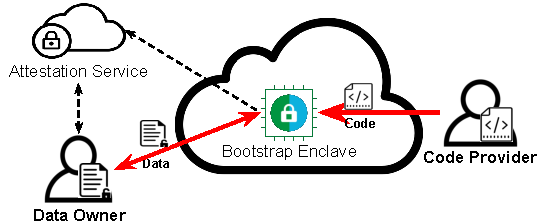
\includegraphics[scale=0.72]{figures/fg-deflection-model.pdf}}
\caption{The \textsc{Deflection} model}\label{fg-cat}
\vspace{-10pt}
\end{figure}
%\weijie{a new figure, to show the trust chain}

%\vspace{3pt}\noindent\textbf{The CAT model}.
\subsection{The Delegation Model}

%The interactions among 4 parties are described as follows.

\vspace{3pt}\noindent\textbf{Attestation service}. Attestation \DIFdelbegin \DIFdel{service }\DIFdelend \DIFaddbegin \DIFadd{Service (AS) }\DIFaddend assists in the remote attestation process by helping the data owner verify the quote generated by an enclave, as performed by the Intel attestation service for SGX. 

%We assume a standard IAS as in Intel's attestation model who verifies the quote and generates the attestation report. 

\vspace{3pt}\noindent\textbf{Bootstrap enclave}. The bootstrap enclave is a built-in control layer on the software stack, hosted by the code provider or a third party cloud  (see Figure~\ref{fg-cat}). Its code is public and initial state is measured by hardware for generating an attestation quote, which is later verified by the data owner with the help of the AS. This software layer is responsible for establishing security channels with enclave users, authenticating and dynamically loading the binary of the target program from the code provider and data from its owner. \DIFdelbegin \DIFdel{Further it }\DIFdelend \DIFaddbegin \DIFadd{It further }\DIFaddend verifies the code to ensure its compliance with predefined security policies before bootstrapping the computation. During the computing, it also controls the data entering or exiting the enclave, e.g., through SGX ECalls/OCalls to perform data sanitization.
    % I want to demonstrate: the loaded code is not allowed to perform OCALL and the ECALL will not reach the loaded code directly. The interfaces are controlled by the bootstrap enclave.

\vspace{3pt}\noindent\textbf{Data owner}. The data owner uploads sensitive data \DIFdelbegin \DIFdel{(e.g., personal images) }\DIFdelend to use in-enclave services \DIFdelbegin \DIFdel{(e.g., an image classifier) }\DIFdelend and intends to keep her data secret during the computation. 
\DIFdelbegin \DIFdel{To this end, the owner runs a remote attestation with the enclave to verify the code of the bootstrap enclave, and sends in data through a secure channel only when convinced that the enclave is in the right state so expected policy compliance check will be properly performed on the target binary from the code provider. 
}%DIFDELCMD < \ignore{
%DIFDELCMD < Note that here we only consider the scenario that the data owner is the only recipient of the output of the enclave service, though the CAT model can be extended to support the application involving multiple data owners and a separate data user.  
%DIFDELCMD < }
%DIFDELCMD < %%%
%DIF < Note that there could be more than one data owner to provide data.  
\DIFdelend 

%Depending on applications, there could be more than one owners to send in data. who feed data into the enclave and would like to keep the data from leaking out of the enclave. For this purpose they initiate a remote attestation by sending an attestation request challenge to the enclave developer, inspect and verify the code of the bootstrap enclave by checking the remote attestation report. If they are convinced the bootstrap enclave can guarantee the predefined policies are applied to the loaded code, they can send the data (in encrypted form) to the bootstrap enclave.

\vspace{3pt}\noindent\textbf{Code provider}. The code provider (owner) can be the service provider, and in this case, her target binary (the service code) can be directly handed over to the bootstrap enclave for compliance check. 
%In general, however, the code provider is a different party and may not trust the cloud platform. 
So, similar to the data owner, she can also request a \revise{flexible/portable} remote attestation to verify the bootstrap enclave before delivering her binary to the enclave for a compliance check. 

\DIFaddbegin \vspace{3pt}\noindent\textbf{\DIFadd{Key agreement procedure}}\DIFadd{.
Both parties, a service provider (data owner) and a remote user (code provider), inspect and agree on the implementation details of the bootstrap enclave. The data owner and the code provider can both attest that the bootstrap loader is correctly running on SGX platforms using remote/local attestation. In particular, data owner and code provider both generate a measurement of the bootstrap enclave, which acts as the trust anchor of their agreement and is required for verification during SGX remote/local attestation.
}

\DIFadd{After the two attestations are done and shared session keys are negotiated by Diffie–Hellman key exchange, all messages can be transferred through the two trusted channels.
Since the data owner already knows the measurement/hash of the service code. The bootstrap enclave first extracts and verifies the measurement/hash of the service code, and then sends the measurement/hash to the data owner. After the data owner is sure about the authenticity of the service code, she can begin to feed data into the service.
}

\DIFaddend % for 11 page limit
\ignore{
\vspace{3pt}\noindent\textbf{Use Cases}.
%\weijie{other portable usage, e.g., enclave migration}
For the example in the introduction, through CAT, a  pharmaceutical company can run its proprietary algorithm inside an enclave hosting patient medical records, without exposing the algorithm but can still ensure the hospital (the data owner) the compliance of its data use with the hospital's privacy policy. As an example, the CAT model can enable a more privacy-preserving credit evaluation service, in which a customer's transactions are only exposed to an enclave running the credit evaluation code in compliance with a set of public privacy-protection rules (such as GDPR).
We consider confidential computing as a service (\textit{CCaaS}) as a privacy extension of today's online data processing services like machine-learning as a service~\cite{russinovich2017introducing}. CCaaS is hosted by the party that operates its own target binary on the data provided by its owner (e.g., an online image classifier to label uploaded user photos). \textit{The outcome of the computation will be sent back to the data owner}. Here, the target binary cannot be released for verification so needs to go through an in-enclave compliance check.
\weijie{code vetting}
}



\ignore{
\vspace{2pt}\noindent\textbf{Sensitive genome data analysis}. Since genetic and health information is extremely sensitive, users may not feel comfortable with the company keeping their data. Meanwhile, a bio-tech companies that owns the intellectual property of its technology would like to use a confidential algorithm to process the data. In this scenario, people upload their genes for private computation that can be outsourced and protected in CAT-SGX. Basic sequence generation and alignment algorithms can be widely used in reads mapping and GATK softwares, while a sequence generation/alignment algorithm often takes strings as an input while gives out strings as ouput. During the confidential service, CAT-SGX keeps the label of genes and the intermediate variables, then forwards the result back to the user when finished. 


\vspace{2pt}\noindent\textbf{Personal credit score analysis}. Consider a bank or a credit agency that provides different levels of loan transactions before it evaluates each applicant's financial status. Then, credit scoring is a typical application that needs to be protected more carefully - both the credit card holder's cost calendar and card issuer's scoring algorithm need to be kept secret. 
The input file contains users' history records and the output is a prediction whether the bank should approve the next transaction. In this case, CAT-SGX only allows two-bytes output to in the score and one bit (bool) to indicate whether the bank should approve or decline the transaction.
}


%could verify the code of the bootstrap enclave through remote attestation. Only after they believe that the bootstrap enclave guarantees the predefined policies, the code can be sent into the bootstrap enclave secretly.

% In order to solve the problem of private algorithm and data, both distrustful parties could utilize secure hardware enclaves. Here, we give some definitions. A Data Owner (DO) refers to an entity who has privacy-sensitive inputs. A Service Provider (SP) refers to an entity who has private algorithms. A Enclave Developer (ED) works with the hardware owner (HO), managing its own computational power and maintaining the hardware.



\subsection{Guidelines}
\label{subsec-challenges} 

To instantiate a \textsc{Deflection} System on a real-world TEE such as SGX, we expect the following requirements to be met by the design: 

%At the core of instantiating the CAT model is the design of the bootstrap enclave who is responsible for enforcing the privacy and security policies. We list the design goals to enable a secure and efficient bootstrap enclave.

\vspace{3pt}\noindent\textbf{Minimizing TCB and resource consumption}.\label{challenge-tcb}\label{challenge-size} 
Today's TEEs operate under resource constraints.  Particularly, SGX is characterized by \DIFdelbegin \DIFdel{limited EPC}\DIFdelend \DIFaddbegin \DIFadd{a limited Enclave Page Cache (EPC)}\DIFaddend . To maintain reasonable performance, we expect the software stack of the \textsc{Deflection} model \DIFdelbegin \DIFdel{controls }\DIFdelend \DIFaddbegin \DIFadd{to control }\DIFaddend its resource use. 
\DIFdelbegin \DIFdel{The bootstrap enclave is responsible for enforcing security and privacy policies and for controlling the interfaces that import and export code/data for the enclave. So it is critical for trust establishment and needs to be kept as compact as possible for code inspection or verification~\mbox{%DIFAUXCMD
\cite{mccune2008flicker}}\hspace{0pt}%DIFAUXCMD
.  
}\DIFdelend %DIF >  The bootstrap enclave is responsible for enforcing security and privacy policies and for controlling the interfaces that import and export code/data for the enclave. So it is critical for trust establishment and needs to be kept as compact as possible for code inspection or verification~\cite{mccune2008flicker}.  

\vspace{3pt}\noindent\textbf{Controlling portable code loading}.\label{challenge-dep} The target binary is dynamically loaded and inspected by the bootstrap enclave. However, the binary may further sideload other code during its runtime. 
%Some TEE hardware, SGX in particular, does not allow dynamic change to enclave page's RWX properties. 
So the target binary, itself loaded dynamically, is executed on the enclave's heap space. Preventing it from sideloading requires a data execution prevention (DEP) scheme to guarantee the W $\oplus$ X privilege.

%current SGX hardware, dynamically changing the RWX properties of enclave pages are not supported. So the loaded program will be executed on enclave's heap space, and we need a fine data execution prevention (DEP) scheme to guarantee W $\oplus$ X privilege.% and isolates security-sensitive data structures from adversaries.

    % Leveraging PCC on program verification could greatly relieve the burden on the code consumer's side - PCC moves most daunting work to the code producer. However, we still need to further improve the performance of our design because there are too many objects (memory write operations and indirect branches) that we have to analyze.
    %\textit{Limited computing resources}. SGX has only a limited memory space. Considering the typical usages of SGX would also occupy tens of MBs of memory, doing confidentiality analysis would be a difficult task. The TCB of the whole verifying system inside the enclave should be as thin as possible. 
    %Also, how to reduce the amount of proof size for verification needs to be dealt with. Thus, we should build a lightweight checking scheme to simplify the verifier/checker with the help of the compiler, and optimize the compiler to generate as less proof as possible.

\vspace{3pt}\noindent\textbf{Preventing malicious control flows}.\label{challenge-cfi} 
Software stack should be designed to prevent the code from escaping policy enforcement by redirecting its control flow or tampering with the bootstrap enclave's critical data structures. Particularly, previous work shows that special instructions like ENCLU could form unique gadgets for control flow \DIFdelbegin \DIFdel{redirecting}\DIFdelend \DIFaddbegin \DIFadd{redirection}\DIFaddend ~\cite{biondo2018guard}, which therefore need proper protection. 

\vspace{3pt}\noindent\textbf{Minimizing performance impact}.\label{challenge-perf} In all application scenarios, the data owner and the code provider expect a quick turnaround from code verification. Also the target binary's performance should not be significantly undermined by the runtime compliance check. 

%It is also important in many scenarios to reduce the time for checking the policy compliance and to induce low run-time overhead for the computation. 



\subsection{Threat Model}
\label{subsec-threat}

\DIFdelbegin \DIFdel{The delegation model is meant to establish trust between the enclave and the code provider, as well as the data owner, under the following assumptions: 
}\DIFdelend %DIF >  The delegation model is meant to establish trust between the enclave and the code provider, as well as the data owner, under the following assumptions: 

%To demonstrate how to instantiate the CAT model, in the rest of the paper we consider a specific application scenario, i.e., privacy preserving online data processing (Scenario 1 in Sec.~\ref{subsec-scenarios}). As shown in Sec.~\ref{subsec-motivation}, many real world privacy preserving data processing tasks fall into this scenario. As described earlier for Scenario 1, the user (i.e., the data provider) submits her sensitive data to a service provider (i.e., the code owner) for data processing tasks. In our threat model, we make the following assumptions.

\vspace{2pt}\noindent$\bullet$ We do not trust the service code (target binary) and the platform hosting the enclave. In CCaaS, the platform may deliberately run vulnerable code to exfiltrate sensitive data, by exploiting \DIFdelbegin \DIFdel{the }\DIFdelend known vulnerabilities during \DIFaddbegin \DIFadd{the }\DIFaddend computation. 
%We trust data owner.
%The binary can also leak the data through a covert channel (e.g., page fault~\cite{xu2015controlled}).   

%\hongbo{Out of our scope: data owner infer code by inspecting the output}

%\vspace{2pt}\noindent$\bullet$ We assume the data owner (service user) is benign. Data provider would not use specially-crafted data to learn about the operation of the secret code given the output.

%\weijie{we do not consider other kinds of leakage such as DOP attack? or the data owner would try to steal the service code. }


%The service provider may (intentionally) write vulnerable service code which causes the leakage of the users' data, e.g., the enclave may be compromised by another user with memory corruption attacks. The service code can even collude with the SGX-enabled platform owned and controlled by the attacker, e.g., through covert channels (such as page faults etc.). 

\ignore{
\weijie{out of scope} \vspace{2pt}\noindent$\bullet$ Our current implementation of CAT-SGX focuses on privacy compliance at this time, and we do not examine the functionalities of the target binary. We believe the design can be extended to ensure other properties of the program. Also, although TEE is designed to prevent information leaks to the untrusted OS, denial of service can still happen, which is outside the scope of the model. }


%\vspace{2pt}\noindent$\bullet$ Under the untrusted service provider, \revise{our method can be used to guarantee the correctness of the computation. However, since the current implementation of CAT-SGX is not meant to inspect the functionalities of the target binary, we only care about the privacy compliance at this time.}
%Since the service provider is untrusted, our design does not intend to guarantee the correctness of the results returned to the users. The service users can refuse to pay for the service or turn to other service providers if the results are inferior. This is similar as Denial-of-Service (DoS) attacks which are also out of scope.

\vspace{2pt}\noindent$\bullet$ We assume that the code of the bootstrap enclave can be inspected to verify its functionalities and correctness.  Also we consider the TEE hardware, its attestation protocol, and all underlying cryptographic primitives to be trusted.  


\DIFdelbegin %DIFDELCMD < \vspace{2pt}\noindent%%%
\DIFdel{$\bullet$ Our model is meant to protect data and code against different kinds of information leaks, not only explicit but also implicit.  However, side channel in a user-land TEE (like SGX) is known to be hard to eliminate, which all existing SGX runtimes (including container~\mbox{%DIFAUXCMD
\cite{arnautov2016scone}}\hspace{0pt}%DIFAUXCMD
, sandbox~\mbox{%DIFAUXCMD
\cite{hunt2018ryoan}}\hspace{0pt}%DIFAUXCMD
, interpreter~\mbox{%DIFAUXCMD
\cite{wang2019towards} }\hspace{0pt}%DIFAUXCMD
and others) fail to address. So our design for instantiating the model on SGX (Section~\ref{subsec-policies}) just aims to make the first step towards closing of this attack surface, mitigating some types of side-channel threats.  
}\DIFdelend %DIF >  \vspace{2pt}\noindent$\bullet$ Our model is meant to protect data and code against different kinds of information leaks, not only explicit but also implicit.  However, side channel in a user-land TEE (like SGX) is known to be hard to eliminate, which all existing SGX runtimes (including container~\cite{arnautov2016scone}, sandbox~\cite{hunt2018ryoan}, interpreter~\cite{wang2019towards} and others) fail to address. So our design for instantiating the model on SGX (Section~\ref{subsec-policies}) just aims to make the first step towards closing of this attack surface, mitigating some types of side-channel threats.  

%Besides, we assume the bootstrap enclave code can be inspected (or formally verified) by the users through remote attestation, so that it is trusted to be functional as designed. We trust the SGX hardware and the Intel's attestation protocol as well as the cryptographic algorithms underneath. The mutual authentication between the users and service provider is orthogonal to the design and is omitted in the paper.

%\weijie{The data provider is relatively benign and won't do things that jeopardizes data privacy of its own, e.g., sending some malicious input (triggering unexpected attacks) into the code. }

% =====================================================================

    
    
    
    
    
    
    
    
%---------------------------------------------------------------------------------------------------------------


\ignore{

\section{Confidential Attestation}\label{sec-CAT}
%\vspace{3pt}\noindent\textbf{Motivating Example}.

\subsection{Motivating Example}\label{subsec-motivation}

Consider a company providing data-processing services, such as image editing (Pixlr), tax preparation (TurboTax), personal health analysis (23andMe) and deep learning inference as a service, the users need to disclose their sensitive data, such as images, tax documents, and health data, to leverage the convenience and expertise of these services. The user can acquire the data processing performed inside an SGX enclave, and further, verify the enclave code through remote attestation to prevent unintended data disclosure. However, the service provider may not want to disclose the enclave code to the user for verification due to intellectual property reasons, in which case the SGX attestation model fails to fulfill the privacy requirement of both the user (i.e. the data owner) and the service provider.

In this section, we propose the \textit{Confidential ATtestation} (CAT) model to allow the data owner to verify that the enclave code satisfies predefined privacy and security policies without undermining the privacy of the enclave code.
We enumerate several application scenarios that could benefit from the proposed CAT model. We will further list the design goals in designing a practical CAT model in the context of Intel SGX, as well as the threat model considered in the paper. 

%Aiming to complete a system that can flexibly verify whether the code leaks data on SGX platforms, we propose Confidential Attestation. This technology can be used in different situations.
%In particular, we will enumerate all technical challenges needed to be overcome during building such a system, and will elaborate the threat model during achieving all purposes of our design.

%The service provider often has secret algorithms or business logic that can not be exposed. As an entity that needs/should to compute a secret value, it may be willing to secure the private algorithm during delivery. Meanwhile, the service provider could sell the intelligent property to a user who wants to process the secret data for a trustworthy and correct result.

%From Intel: With a bit of hand waving one could envision a 'proprietary' code module which is symmetrically encrypted and thus protected outside the context of an enclave.   In this model one still needs a 'bootstrap' enclave which has to have access to the encryption material needed to authenticate and decrypt the code/data which is being dynamically loaded.  That leaves you back at the need to establish a security context between the 'bootstrap' enclave and the authority/context which has prepared the protected material for ingress into the enclave.

%\vspace{3pt}\noindent\textbf{The CAT model}.
\subsection{The CAT model}

There are 4 parties involved in the CAT model.

%\vspace{3pt}\noindent\textbf{The enclave developer}. It provides the code of the bootstrap enclave (see below), which can be made public. Then it conducts the Intel's attestation model as an ISV on behalf of the data providers and the code providers (see below). Specifically it accepts the attestation request challenge and forwards it to the enclave, then it forwards the quotes to the IAS to get the attestation report. At last it forwards the attestation report to the party who initiates the remote attestation.
%\hongbo{Why should enclave developer appears in the CAT model? During the lifetime of the bootstrap enclave/service code, the developer will not be in the computation task. The attestation will be done by the bootstrap enclave(not the developer). Maybe platform is more appropriate}

\vspace{3pt}\noindent\textbf{The IAS}. We assume a standard IAS as in Intel's attestation model who verifies the quote and generates the attestation report. 

\vspace{3pt}\noindent\textbf{The bootstrap enclave}. It is the initial code built into the enclave, which is measured by the hardware to generate the measurement report. It is responsible to authenticate and dynamically load the code and data for the computation to be conducted. It then verifies the code and data is compliant to predefined policies and bootstraps the computation. It is responsible for establishing protected communication channels, and audit the ECalls/OCalls to sanitize the data sent to or received from outside of the enclave.
    % I want to demonstrate: the loaded code is not allowed to perform OCALL and the ECALL will not reach the loaded code directly. The interfaces are controlled by the bootstrap enclave.

\vspace{3pt}\noindent\textbf{The data providers}. Depending on the applications, there can be multiple data providers who feed data into the enclave and would like to keep the data from leaking out of the enclave. For this purpose they initiate a remote attestation by sending an attestation request challenge to the enclave developer, inspect and verify the code of the bootstrap enclave by checking the remote attestation report. If they are convinced the bootstrap enclave can guarantee the predefined policies are applied to the loaded code, they can send the data (in encrypted form) to the bootstrap enclave.

\vspace{3pt}\noindent\textbf{The code providers}. Similar as the data providers, code provider/owner could verify the code of the bootstrap enclave through remote attestation. Only after they believe that the bootstrap enclave guarantees the predefined policies, the code can be sent into the bootstrap enclave secretly.

% In order to solve the problem of private algorithm and data, both distrustful parties could utilize secure hardware enclaves. Here, we give some definitions. A Data Owner (DO) refers to an entity who has privacy-sensitive inputs. A Service Provider (SP) refers to an entity who has private algorithms. A Enclave Developer (ED) works with the hardware owner (HO), managing its own computational power and maintaining the hardware. 
\subsection{Application Scenarios}\label{subsec-scenarios}

In the following, we enumerate several application scenarios that could benefit from the proposed CAT model. 
%\weijie{code and data should be encrypted sometimes for such three scenarios.}
%\vspace{3pt}\noindent\textbf{Examples.}

\begin{figure}[htbp]
\begin{center}
\centerline{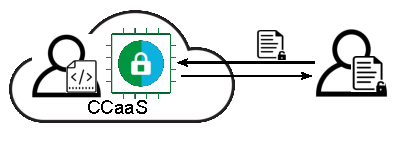
\includegraphics[scale=0.72]{figures/fg-scenario-1.pdf}}
\caption{Scenario 1}\label{fg-scenario_1}
\end{center}
\end{figure}


\weijie{change the name of scenarios to: confidential computing as a service, confidential data as a service, etc.}

\vspace{3pt}\noindent\textbf{Scenario~\ref{fg-scenario_1}: Privacy preserving online data processing service}. As the motivating example (Sec.~\ref{subsec-motivation}) shows, the data-processing service (i.e., the bootstrap enclave) is hosted on an SGX-enabled platform owned by the service provider (i.e., the code provider), while the user (i.e., the data provider) sends her encrypted sensitive data for processing. The result will be sent back to the data provider (possibly in encrypted form). As such, the user would like that the bootstrap enclave can enforce the security policy that her data would never leave the enclave.
%\hongbo{In these figures, is enclave developer denotes the cloud? I think it should be SGX-enabled platform.}

\begin{figure}[htbp]
\centerline{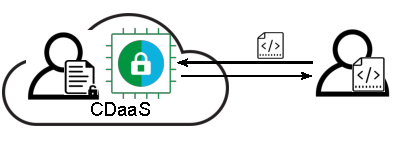
\includegraphics[scale=0.72]{figures/fg-scenario-2.pdf}}
\caption{Scenario 2}\label{fg-scenario_2}
\end{figure}

\vspace{3pt}\noindent\textbf{Scenario~2: Privacy preserving online data as a service}. In this scenario, the data-as-a-service (i.e., the bootstrap enclave) is hosted on an SGX-enabled platform owned by the data provider. A user (i.e., the code owner) who would like to conduct computation (such as genome analysis) on the data sends her sensitive code via a secure channel . The result will be sent back to the code provider (possibly in encrypted form). As such, the user would like that the bootstrap enclave can enforce the security policy that the data used are not faked or impure, and her code will not be unintended redirected so that the result is reliable.

\begin{figure}[htbp]
\centerline{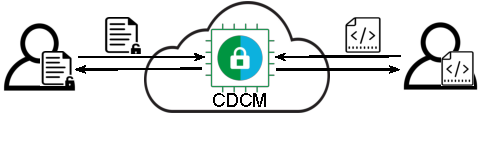
\includegraphics[scale=0.72]{figures/fg-scenario-3.pdf}}
\caption{Scenario 3}\label{fg-scenario_3}
\end{figure}

\vspace{3pt}\noindent\textbf{Scenario~3: Privacy preserving online data market}. In this scenario, a data market platform (i.e., the bootstrap enclave) is hosted on a third party.
%besides the data user (i.e., the code provides) and data owner (i.e., the data providers). 
The data owner uploads her encrypted data to the platform so that she gets paid if the data is used. The data user uploads her code (e.g. genome analysis) also secretly to be computed on people's data satisfying some preset conditions. As such, besides enforcing the confidentiality of both the code and data, the data owner would like to ensure that she gets paid as long as the data is used, while the data user want to ensure that she's not overcharged.

Besides the above scenarios, CAT may be used in more applications, such as privacy preserving smart contract, etc.

%\vspace{3pt}\noindent\textbf{Technical challenges}.
\subsection{Design goals}
\label{subsec-challenges} 
At the core of instantiating the CAT model is the design of the bootstrap enclave who is responsible for enforcing the privacy and security policies.
We list the design goals to enable a secure and efficient bootstrap enclave.

\vspace{3pt}\noindent\textbf{Minimizing the Trusted Computing Base (TCB)}.\label{challenge-tcb} 
    In the CAT model the bootstrap enclave is responsible for enforcing the security and privacy policies and to control the interfaces between the loaded code/data and outside of the enclave. The trust built by the CAT model will collapse once it is compromised. It is essential to control the size of the bootstrap enclave and that it can be (formally) verified in the future.

\vspace{3pt}\noindent\textbf{Reducing the memory consumption}.\label{challenge-size} 
    There are limited EPC memory that could be used by the SGX enclave. Considering that the data-processing computation itself consume considerable memory, the design needs to reduce the memory cost adequately.

\vspace{3pt}\noindent\textbf{Confining the (untrusted) loaded code}.\label{challenge-dep} On current SGX hardware, dynamically changing the RWX properties of enclave pages are not supported. So the loaded program will be executed on enclave's heap space, and we need a fine data execution prevention (DEP) scheme to guarantee W $\oplus$ X privilege.% and isolates security-sensitive data structures from adversaries.

    % Leveraging PCC on program verification could greatly relieve the burden on the code consumer's side - PCC moves most daunting work to the code producer. However, we still need to further improve the performance of our design because there are too many objects (memory write operations and indirect branches) that we have to analyze.
    %\textit{Limited computing resources}. SGX has only a limited memory space. Considering the typical usages of SGX would also occupy tens of MBs of memory, doing confidentiality analysis would be a difficult task. The TCB of the whole verifying system inside the enclave should be as thin as possible. 
    %Also, how to reduce the amount of proof size for verification needs to be dealt with. Thus, we should build a lightweight checking scheme to simplify the verifier/checker with the help of the compiler, and optimize the compiler to generate as less proof as possible.

\vspace{3pt}\noindent\textbf{Preventing malicious control flows}.\label{challenge-cfi} 
    Previous work shows that special instructions in SGX like ENCLU would make unique gadgets for control flow redirecting attacks.
    Since the loaded code can not be trusted, the design needs to prevent code from escaping the policy enforcement by redirecting the control flow and tampering the security-sensitive data structures of the bootstrap code.
    %code control flow hijacking techniques to compromise
    %Although we can use SGX's Remote Attestation (RA) to ensure the integrity of our verifier/checker, there can be many control flow hijacking techniques to compromise the verifier and bypass the checks. 
     %So a more thorought CFI policies should be executed to prevent various malicious control flow redirecting within the untrusted service code.
   % \item \textit{Dynamic code loading and data execution protection}.\label{challenge-3} Normal x86 binaries built outside the enclave can not be simply running inside, due to restrictions caused by Intel SGX. To enable verifying the service provider’s code yet without knowing the code itself, a loader in enclave could be built so that the loader do the verification and be attested by remote user using Intel SGX’s RA. But how to design a practical loader for loading/relocating binaries dynamically? Therefore, we need a good way to assemble the binary using our code generator and load the relocatable file after the loader is initialized. In the meantime, since the loaded program will be executed on enclave's heap space, we also need a fine DEP plan to guarantee W $\oplus$ X privilege and isolates security-sensitive data structures from adversaries.

\vspace{3pt}\noindent\textbf{Performance considerations}.\label{challenge-perf} It is also important in many scenarios to reduce the time for checking the policy compliance and to induce low run-time overhead for the computation. 

%\vspace{3pt}\noindent\textbf{Threat model}. 
\subsection{Threat model}
\label{subsec-threat}
%In this paper we assume a strong adversary in the CAT model, i.e., the code providers and data providers do not trust each other. 
To demonstrate how to instantiate the CAT model, in the rest of the paper we consider a specific application scenario, i.e., privacy preserving online data processing (Scenario 1 in Sec.~\ref{subsec-scenarios}). As shown in Sec.~\ref{subsec-motivation}, many real world privacy preserving data processing tasks fall into this scenario. 
%We stress that instantiating the CAT model in the other application scenarios are important future works.
As described earlier for Scenario 1, the user (i.e., the data provider) submits her sensitive data to a service provider (i.e., the code owner) for data processing tasks. In our threat model, we make the following assumptions.

%Before the discussion of how we design a practical Privacy-preserving TEE, a threat model could be built for better define the scope of the problem we need to solve. 

\vspace{2pt}\noindent$\bullet${ The service code and the SGX-enabled host platform are not trusted.} The service provider may (intentionally) write vulnerable service code which causes the leakage of the users' data, e.g., the enclave may be compromised by another user with memory corruption attacks. The service code can even collude with the SGX-enabled platform owned and controlled by the attacker, e.g., through covert channels (such as page faults etc.). 

%to do whatever they can to steal the data owner’s sensitive information. But we believe in Intel SGX and its RA protocol, which could be seen as a trusted third party.


%\hongbo{Do we need to mention the cloud computation platform is also untrusted?}
\vspace{2pt}\noindent$\bullet$ Since the service provider is untrusted, our design does not intend to guarantee the correctness of the results returned to the users. The service users can refuse to pay for the service or turn to other service providers if the results are inferior. This is similar as Denial-of-Service (DoS) attacks which are also out of scope.

\vspace{2pt}\noindent$\bullet$ Besides, we assume the bootstrap enclave code can be inspected (or formally verified) by the users through remote attestation, so that it is trusted to be functional as designed. We trust the SGX hardware and the Intel's attestation protocol as well as the cryptographic algorithms underneath. The mutual authentication between the users and service provider is orthogonal to the design and is omitted in the paper.

%\vspace{2pt}\noindent$\bullet$\textit{The data is encrypted and intact before the enclave starts to run the data-processing application.} Intel SGX and its built-in toolsets can make both the service provider’s code and user’s data loaded into an enclave securely via RA and key exchange. And if necessary, service provider could apply some differential privacy techniques and add certain noisy to protect the data from inference attacks.
    %As discussed earlier the loaded code cannot perform Ocalls directly, and we assume that all ECalls/OCalls will be audited by the bootstrap enclave. 
    %Since all the bridge functions should be public for normal use, it makes sense that we can make such assumption in this service-oriented scenarios. And if necessary, service provider could add certain noisy to protect the data from inference attacks.
    %\item Currently, we do not consider side channels or covert channels between the enclave code and the outside world. In this paper, we are confined to verifying simple confidentiality properties and do not handle complex adversary models like those involving side-channels.\wenhao{remove this item}
}

    
    